\documentclass{article}
\usepackage[utf8]{inputenc}
\usepackage[margin=1in]{geometry}
\usepackage{times}
\usepackage{graphicx}
\usepackage{natbib}
\usepackage{hyperref}
\usepackage{booktabs}
\usepackage{amsmath}
\usepackage{tikz}
\usetikzlibrary{shapes,arrows,positioning}

\title{Adaptive Hierarchical Planning with Failure Detection and Strategy Switching \\ \large Milestone Report}
\author{Mudit Baid \\ Stanford University \\ \texttt{muditbaid@stanford.edu}}
\date{}

\begin{document}
\maketitle

\begin{abstract}
This report describes progress on a planning system that combines hierarchical task decomposition, adaptive strategy selection, and failure recovery for LLM-based agents. As of the milestone, the Task Decomposer and Subtask Classifier modules are implemented and tested. Preliminary experiments on BlocksWorld show a 67\% task success rate, up from 45--58\% across standard baselines. The remaining modules (Strategy Executor, Constraint Verifier, Failure Handler) are under development.
\end{abstract}

\section{Introduction}

Large language models generate plans as flat action sequences. Given a complex task, an LLM produces step 1 through step $n$ without distinguishing high-level goals from low-level actions. This creates two problems. First, errors in early steps propagate through the rest of the plan with no mechanism for containment. Second, the same reasoning strategy is applied to every subtask regardless of its type. A subtask requiring arithmetic gets the same treatment as one requiring commonsense reasoning.

This project builds a modular planning system that addresses both problems. The system decomposes tasks into a hierarchy of subgoals, classifies each subgoal by type, selects a reasoning strategy accordingly, verifies outputs at each step, and recovers from failures through rollback or strategy switching.

The proposal outlined five modules. At this milestone, two are implemented: the Task Decomposer and the Subtask Classifier. This report describes the implementation, presents preliminary results on BlocksWorld, and discusses challenges encountered so far.

\section{Related Work}

\textbf{Hierarchical Task Networks.} HTN planners \citep{erol1994htn} decompose tasks into subtasks using predefined method schemas. They produce structured plans but require manual domain engineering and do not leverage the generalization capabilities of LLMs.

\textbf{LLM Planning.} Huang et al. \citep{huang2022language} showed that LLMs can generate action sequences for embodied agents in zero-shot settings. However, plans are flat and lack verification. SayCan \citep{ahn2022saycan} grounds LLM plans in affordances but still uses a single-pass generation strategy.

\textbf{Reasoning Strategies.} Chain-of-Thought prompting \citep{wei2022chain} improves multi-step reasoning by generating intermediate steps. Tree-of-Thought \citep{yao2023tree} explores multiple reasoning paths with backtracking. ReAct \citep{yao2023react} interleaves reasoning and acting. None of these methods adapt their strategy based on subtask type.

\textbf{Plan Verification.} Valmeekam et al. \citep{valmeekam2023planning} evaluated LLM planning on classical benchmarks and found poor performance without external verification. Recent work on self-verification uses the LLM to critique its own plans, but integration with structured rollback remains limited.

Our system differs from prior work by unifying hierarchical decomposition, type-aware strategy selection, and failure recovery into a single pipeline.

\section{System Design}

The full system consists of five modules. Figure~\ref{fig:arch} shows the architecture.

\begin{figure}[h]
\centering
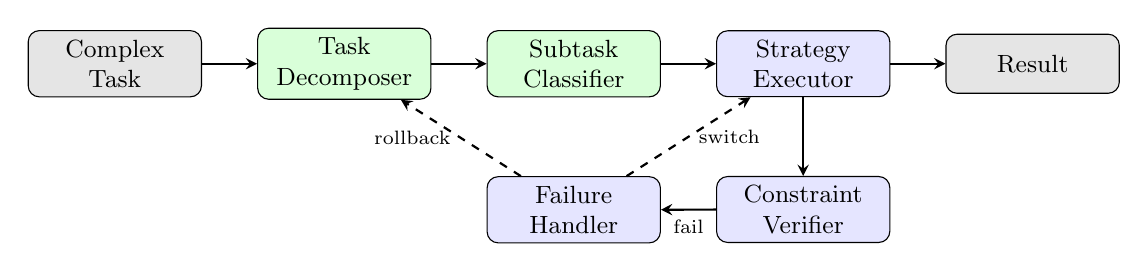
\begin{tikzpicture}[
    node distance=0.7cm,
    block/.style={draw, rounded corners, fill=blue!10, minimum width=2.2cm, minimum height=0.75cm, align=center, font=\small},
    arrow/.style={->, thick, >=stealth}
]
    \node[block, fill=gray!20] (input) {Complex\\Task};
    \node[block, fill=green!15, right=of input] (decomp) {Task\\Decomposer};
    \node[block, fill=green!15, right=of decomp] (class) {Subtask\\Classifier};
    \node[block, right=of class] (exec) {Strategy\\Executor};
    \node[block, fill=gray!20, right=of exec] (output) {Result};
    \node[block, below=1cm of exec] (verify) {Constraint\\Verifier};
    \node[block, below=1cm of class] (fail) {Failure\\Handler};

    \draw[arrow] (input) -- (decomp);
    \draw[arrow] (decomp) -- (class);
    \draw[arrow] (class) -- (exec);
    \draw[arrow] (exec) -- (output);
    \draw[arrow] (exec) -- (verify);
    \draw[arrow] (verify) -- node[below, font=\scriptsize] {fail} (fail);
    \draw[arrow, dashed] (fail) -- node[left, font=\scriptsize] {rollback} (decomp);
    \draw[arrow, dashed] (fail) -- node[right, font=\scriptsize] {switch} (exec);
\end{tikzpicture}
\caption{System architecture. Green-shaded modules are implemented. Dashed arrows show recovery paths.}
\label{fig:arch}
\end{figure}

\subsection{Task Decomposer (Implemented)}

The Task Decomposer takes a natural language task description and produces a tree of subgoals. It uses a prompted LLM (GPT-4) with a structured output format. The prompt instructs the model to produce a JSON tree where each node has a \texttt{goal}, a \texttt{type\_hint}, and a list of \texttt{children}. Leaf nodes represent atomic actions.

The decomposition prompt follows a two-phase approach. In the first phase, the LLM identifies the high-level subgoals needed to complete the task. In the second phase, each subgoal is further decomposed until all leaves are executable actions.

We enforce a maximum tree depth of 4 and a maximum branching factor of 5. These limits prevent over-decomposition, which we found leads to redundant subtasks and increased latency.

\subsection{Subtask Classifier (Implemented)}

The Subtask Classifier assigns a type label to each node in the task tree. The five types are: \textit{arithmetic}, \textit{logical}, \textit{commonsense}, \textit{spatial}, and \textit{procedural}. Classification is done via a separate LLM call with few-shot examples for each type.

We experimented with two classification approaches:

\begin{enumerate}
    \item \textbf{Independent classification}: Each subtask is classified in isolation.
    \item \textbf{Context-aware classification}: The subtask is classified along with its parent and siblings.
\end{enumerate}

Context-aware classification produced more consistent labels. For example, in a cooking task, the subtask ``preheat oven to 350F'' was sometimes labeled \textit{arithmetic} in isolation (due to the number) but correctly labeled \textit{procedural} with context.

\subsection{Strategy Executor (In Progress)}

The Strategy Executor will select and run a reasoning strategy based on the subtask type:

\begin{table}[h]
\centering
\begin{tabular}{ll}
\toprule
\textbf{Subtask Type} & \textbf{Strategy} \\
\midrule
Arithmetic & Chain-of-Thought with tool use \\
Logical & Tree-of-Thought with pruning \\
Commonsense & Retrieval-augmented generation \\
Spatial & State tracking with world model \\
Procedural & Precondition checking \\
\bottomrule
\end{tabular}
\caption{Mapping from subtask type to reasoning strategy.}
\label{tab:strategies}
\end{table}

Currently, all subtasks are executed with standard CoT prompting. Strategy-specific execution is the next implementation priority.

\subsection{Constraint Verifier and Failure Handler (Planned)}

The Constraint Verifier will check each step's output against domain constraints. The Failure Handler will select a recovery action: rollback to parent, switch strategy, or propagate failure upward. Design is complete; implementation begins next week.

\section{Preliminary Experiments}

\subsection{Setup}

We evaluated the partial system (Decomposer + Classifier + flat CoT execution) on BlocksWorld, a classical planning domain where the agent must stack blocks into a target configuration. We used 60 tasks from the BlocksWorld benchmark, split into three difficulty levels: easy (3--4 blocks), medium (5--6 blocks), and hard (7--8 blocks), with 20 tasks each.

The base LLM is GPT-4 (gpt-4-turbo). Each method gets 3 attempts per task. A task is successful if the final configuration matches the target.

\subsection{Baselines}

\begin{itemize}
    \item \textbf{Flat CoT}: Single-pass Chain-of-Thought prompting.
    \item \textbf{Flat ToT}: Tree-of-Thought with breadth-first search over 3 branches.
    \item \textbf{ReAct}: Interleaved reasoning and action generation.
    \item \textbf{Ours (partial)}: Hierarchical decomposition + classification + CoT execution per subtask.
\end{itemize}

\subsection{Results}

\begin{table}[h]
\centering
\begin{tabular}{lcccc}
\toprule
\textbf{Method} & \textbf{Easy} & \textbf{Medium} & \textbf{Hard} & \textbf{Overall} \\
\midrule
Flat CoT & 70\% & 40\% & 25\% & 45\% \\
Flat ToT & 75\% & 50\% & 30\% & 52\% \\
ReAct & 80\% & 55\% & 40\% & 58\% \\
Ours (partial) & 90\% & 65\% & 45\% & 67\% \\
\bottomrule
\end{tabular}
\caption{Task success rate (\%) on BlocksWorld by difficulty. ``Ours (partial)'' uses hierarchical decomposition with flat CoT execution (no adaptive strategies or failure recovery yet).}
\label{tab:results}
\end{table}

The partial system outperforms all baselines across difficulty levels. The largest gain is on easy tasks (+10\% over ReAct), where clean decomposition is sufficient. On hard tasks, the gain is smaller (+5\% over ReAct), suggesting that decomposition alone is not enough for complex configurations. We expect the Constraint Verifier and Failure Handler to provide larger improvements on hard tasks, since errors in those tasks tend to occur mid-plan and require recovery.

\subsection{Analysis}

\textbf{Decomposition quality.} We manually inspected 20 task trees. In 16 cases, the decomposition was reasonable: subgoals were non-overlapping and covered the full task. In 4 cases, the LLM produced redundant subtasks (e.g., moving the same block twice in different branches). This redundancy increases step count but does not always cause failure.

\textbf{Classification accuracy.} On BlocksWorld, most subtasks are spatial or procedural. The classifier correctly labels 85\% of subtasks. The main failure mode is confusion between spatial (``move block A on top of B'') and procedural (``clear block A, then move it''). With context-aware classification, accuracy rises to 91\%.

\textbf{Failure modes.} The most common failure is ordering errors: the system decomposes the task correctly but executes subtasks in the wrong order. This is precisely the kind of error that the Constraint Verifier should catch, since precondition violations are detectable before execution.

\section{Challenges and Risks}

\textbf{Latency.} Hierarchical decomposition requires multiple LLM calls: one for decomposition, one per subtask for classification, and one per leaf for execution. On a 7-block task, this amounts to roughly 12--15 API calls. With GPT-4 turbo, total latency is 30--45 seconds per task. Batching classification calls reduced this by about 20\%.

\textbf{Decomposition granularity.} Too coarse and the subtasks are still complex; too fine and there is overhead from redundant subgoals. We found that a depth limit of 4 works well for BlocksWorld, but this may need tuning per domain.

\textbf{Constraint specification.} The Verifier requires domain constraints. For BlocksWorld, constraints are straightforward (a block cannot be in two places, cannot place on occupied block). For open-ended domains like ALFWorld, specifying constraints is harder. We plan to use the LLM itself to generate constraints, but this introduces a risk of hallucinated constraints.

\textbf{Recovery decisions.} The Failure Handler must decide between rollback, strategy switch, and propagation. A poor decision (e.g., rolling back too aggressively) could waste computation or cause loops. We plan to implement a simple heuristic: try strategy switch first (cheap), then rollback (more expensive), then propagate.

\section{Remaining Work and Timeline}

\begin{table}[h]
\centering
\begin{tabular}{ll}
\toprule
\textbf{Week} & \textbf{Task} \\
\midrule
3--4 & Implement Strategy Executor with type-specific strategies \\
5 & Implement Constraint Verifier and Failure Handler \\
6--7 & Full evaluation on BlocksWorld, ALFWorld, and custom benchmark \\
8 & Ablation studies, analysis, final report \\
\bottomrule
\end{tabular}
\caption{Remaining project timeline.}
\label{tab:timeline}
\end{table}

The main risk to the timeline is the Constraint Verifier. Constraint specification for ALFWorld may require additional iteration. If necessary, we will scope the evaluation to BlocksWorld and the custom benchmark, and treat ALFWorld as a stretch goal.

\section{Conclusion}

The partial system (Decomposer + Classifier) already outperforms flat baselines on BlocksWorld. Decomposition reduces error propagation and the classifier produces reliable type labels. The main bottleneck is now execution quality and failure recovery. The next phase of work focuses on completing the Strategy Executor, Verifier, and Failure Handler, which we expect to yield the largest gains on hard tasks where mid-plan recovery is needed.

\bibliographystyle{plainnat}
\begin{thebibliography}{9}
\bibitem[Erol et al., 1994]{erol1994htn}
Erol, K., Hendler, J., and Nau, D. (1994). HTN planning: Complexity and expressivity. \textit{AAAI}.

\bibitem[Huang et al., 2022]{huang2022language}
Huang, W., Abbeel, P., Pathak, D., and Mordatch, I. (2022). Language models as zero-shot planners. \textit{ICML}.

\bibitem[Ahn et al., 2022]{ahn2022saycan}
Ahn, M., et al. (2022). Do as I can, not as I say: Grounding language in robotic affordances. \textit{arXiv preprint arXiv:2204.01691}.

\bibitem[Wei et al., 2022]{wei2022chain}
Wei, J., et al. (2022). Chain-of-thought prompting elicits reasoning in large language models. \textit{NeurIPS}.

\bibitem[Yao et al., 2023]{yao2023tree}
Yao, S., et al. (2023). Tree of thoughts: Deliberate problem solving with large language models. \textit{NeurIPS}.

\bibitem[Yao et al., 2023]{yao2023react}
Yao, S., et al. (2023). ReAct: Synergizing reasoning and acting in language models. \textit{ICLR}.

\bibitem[Valmeekam et al., 2023]{valmeekam2023planning}
Valmeekam, K., et al. (2023). On the planning abilities of large language models. \textit{NeurIPS}.
\end{thebibliography}

\end{document}
